\documentclass{article}

% S\'imbolos
\usepackage{recycle}
\usepackage{amsfonts}

% Figuras
\usepackage{algorithmic}
\usepackage{graphicx}

% Gr\'aficas
\usepackage{tikz}

% Estilo Tikz
\tikzstyle{edge}=[shorten <=2pt, shorten >=2pt,
                  >=stealth, line width=1.1pt]
\tikzstyle{vertex}=[circle, fill=white, draw,
                    minimum size=5pt,
                    inner sep=0pt, outer sep=0pt]

% M\'argenes
\addtolength{\voffset}{-1cm}
\addtolength{\hoffset}{-1.5cm}
\addtolength{\textwidth}{3cm}
\addtolength{\textheight}{2cm}

% Encabezados y Pies de P\'agina
\usepackage{fancyhdr}
% Informaci\'on del Encabezado
\lhead{Teor\'ia de Gr\'aficas II 2021-2 \\
       Tarea 1}
\rhead{Profesor: C\'esar Hern\'andez Cruz \\
       Ayudante: Daniel Garc\'ia Argueta}
% Informaci\'on del Pie de P\'agina
\rfoot{\recycle}
\cfoot{\vspace{-0.8cm}?`Realmente necesitas imprimir esta hoja?}
\lfoot{\recycle}
\pagenumbering{gobble}
\footskip = 50pt
% L\'inea del encabezado
\renewcommand\headrulewidth{1.5pt}
%%%%%%%%%%%%%%%%%%%%%%%%%%%%%%%%%%%%%%%%%%%%%%%%%%%%%%%%%%%%%
%%%%%%%%%%%%%%%%%%%%%%%%%%%%%%%%%%%%%%%%%%%%%%%%%%%%%%%%%%%%%
%%%%%%%%%%          Gr\'afica en encabezado          %%%%%%%%%%
%%%%%%%%%%%%%%%%%%%%%%%%%%%%%%%%%%%%%%%%%%%%%%%%%%%%%%%%%%%%%
%%%%%%%%%%%%%%%%%%%%%%%%%%%%%%%%%%%%%%%%%%%%%%%%%%%%%%%%%%%%%
\makeatletter
\def\headrule{{\if@fancyplain\let\headrulewidth\plainheadrulewidth\fi
\hrule\@height\headrulewidth\@width\headwidth
\vspace{0.1cm}
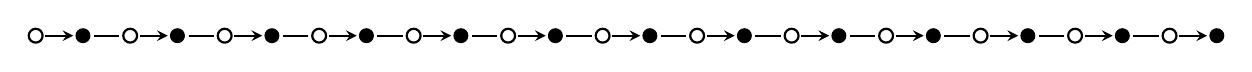
\begin{tikzpicture}
  \begin{scope}[scale=0.6]
   \foreach \x in {0,2,...,24} {
      \node [circle,draw,thick,inner sep=0,minimum size=5pt] (\x) at (\x,0){};
   }
   \foreach \x in {1,3,...,25} {
      \node [circle,draw,fill=black,inner sep=0,minimum size=5pt] (\x) at (\x,0){};
   }
   \foreach \x/\y in {0,2,...,24} {
     \pgfmathsetmacro\result{\x + 1}
     \draw [->,>=stealth,shorten <=3.5pt, shorten >=3.5pt,line width=0.7pt] (\x,0) to (\result,0);
   }
   \foreach \x/\y in {1,3,...,23} {
     \pgfmathsetmacro\result{\x + 1}
     \draw [>=stealth,shorten <=4pt, shorten >=4pt,line width=0.7pt] (\x,0) to (\result,0);
   }
   % \node [inner sep=0,minimum size=5pt] (25.5) at (25.5,-0.05){$\cdots$};
  \end{scope}
\end{tikzpicture}
\vskip-\headrulewidth
\vskip-1.5pt}}
\makeatother
%%%%%%%%%%%%%%%%%%%%%%%%%%%%%%%%%%%%%%%%%%%%%%%%%%%%%%%%%%%%%
%%%%%%%%%%%%%%%%%%%%%%%%%%%%%%%%%%%%%%%%%%%%%%%%%%%%%%%%%%%%%
%%%%%%%%%%%%%%%%%%%%%%%%%%%%%%%%%%%%%%%%%%%%%%%%%%%%%%%%%%%%%
%%%%%%%%%%%%%%%%%%%%%%%%%%%%%%%%%%%%%%%%%%%%%%%%%%%%%%%%%%%%%
%%%%%%%%%%%%%%%%%%%%%%%%%%%%%%%%%%%%%%%%%%%%%%%%%%%%%%%%%%%%%

% Estilo
\pagestyle{fancyplain}

% Macros
\newcommand{\set}[1]{\left\{ #1 \right\}}


\begin{document}

\begin{enumerate}
  \item \textbf{Demuestre que si $D$ es una digr\'afica, entonces su
    condensaci\'on $D^\ast$ es ac\'iclica.}

    Por contradicci\'on, suponga que $D$ es una digr\'afica, $D^\ast$ su condensaci\'on y $C=(C_0,\dots,C_{n-1},C_0)$ un ciclo en ella.. Sea $i\in[n-1]$ y consideremos las componentes $C_i,C_{i+1 mod n}$, ya que $D^\ast$ no tiene lazos, estas son componentes fuertes distintas.

    Veamos que como $(C_i, C_{i+1 modn})\in A(D^\ast)$, por definici\'on de la condensaci\'on aseguramos que existe $v_i\in C_i, w_i\in C_{i+1 modn}$ tales que $(v_i,w_i)\in A(D)$. Luego, para cualquier $u\in C_i$, se tiene que por estar en la misma componente fuertemente conexa que $v_i$, entonces existe una $uv_i$-trayectoria ``$P$'', y de forma an\'aloga, para todo $u'\in C_{i+1 modn}$ existe una $w_iu'$-trayectoria ``$P'$''; de \'esto se concluye que $\forall i\in[n-1]\forall u\in C_i \forall u'\in C_{i+1 modn}$ existe una $uu'$-trayectoria, a saber $uPv_iw_iP'u'$.

  En s\'intesis, cualquier v\'ertice de una componente fuertemente conexa en el ciclo $C$ puede alcanzar, en $D$, a todo v\'ertice de la siguiente componente en $C$. Pero, por la naturaleza c\'iclica de $C$, esto implica que todo v\'ertice de una componente $C_i$, puede alcanzar a todo v\'ertice de otra componente $C_j$, con lo que conclu\'imos que la gr\'afica inducida por la uni\'on $\cup_{i=1}^nC_i$ es fuertemente conexa, lo que es una contradicci\'on al hecho de que $C$ fuera un ciclo.

  \item \textbf{Demuestre que si $D$ es una digr\'afica ac\'iclica, entonces
    tiene un \'unico n\'ucleo.   Adem\'as, a partir de su demostraci\'on
    obtenga un algoritmo para encontrar un n\'ucleo en una digr\'afica
    ac\'iclica.   ?`Qu\'e complejidad tiene su algoritmo?}

    Por inducci\'on sobre $|V|$. Para $|V|=1$ es claro que se cumple, pues el conjunto $V$ es un n\'ucleo y adem\'as es el \'unico.

    Ahora, supongamos que para cualquier digr\'afica ac\'icilica que cumpla $|V|=k$, tiene un \'unico n\'ucleo. Sea $D$ una digr\'afica con $|V|=k+1$, luego, por ser ac\'icilica, $D$ tiene una fuente, denot\'emosla $v$. Veamos que $D'=D-v$ es una digr\'afica ac\'icilica de $k$ v\'ertices, por lo tanto tiene un \'unico n\'ucleo $N'$.

    Si $N^+(v)\cap N'\neq\emptyset$, entonces $N'$ es un conjunto independiente que absorbe a todo v\'ertice de $D$, por lo tanto es un n\'ucleo de $D$; si por otro lado $N^+(v)\cap N'=\emptyset$, entonces ning\'un exvecino de $v$ est\'a en $N'$, y por ser una fuente de $D$, no tiene ning\'un invecino, de aqu\'i se concluye que $N=N'\cup\set{v}$ es un conjunto independiente, y como $N'$ absorbe a todo v\'ertice distinto de $v$, entonces $N$ es un n\'ucleo de $D$.

    Ahora veamos que es \'unico, sea $N_0$ un n\'ucleo cualquiera de $D$, ahora consideremos $N_0-\set{v}$, como $N_0$ absorbe todos los v\'ertices de $D$ y ya que $v$ no tiene invecinos (es decir, ning\'un v\'ertice es absorbido por \'el), se tiene que $N_0-\set{v}$ es un n\'ucleo de $D-v$. Pero por hip\'otesis de inducci\'on \'este n\'ucleo era \'unico era \'unico, entonces $N'=N_0-\set{v}$, finalmente, se puede deducir si $v$ es un elemento de $N_0$ usando los mismos argumentos que usamos para construir $N$, y de \'esta forma el n\'ucleo de $D$ es \'unico.

      \begin{algorithmic}[1]
        \REQUIRE Una gr\'afica ac\'iclica $G$, su conjutno de v\'ertices $V$ y de flechas $A$.
        \ENSURE$K$ el \'unico n\'ucleo de $G$
        \WHILE {$V\neq\emptyset$}
        \FOR {$v\in V$}
        \IF {$v$ es un sumidero de $G$}
        \STATE $K=K\cup\set{v}$
        \STATE borramos a $v$ y a todos sus invecinos del conjunto de v\'ertices $V$
        \STATE $G=[V]$
        \ENDIF
        \ENDFOR
        \ENDWHILE
        \STATE \textbf{Return:} $K$
      \end{algorithmic}

      \'Este algoritmo funciona porque el sumidero de una gr\'afica ac\'iclica siempre debe estar en su n\'ucleo, pues no puede ser absorbido por otro v\'ertice. Luego borramos el sumidero junto con todos los v\'ertices que absorbe, \'esto nos deja con una gr\'afica conformada de v\'ertices ajenos al conjunto $K$ y, al ser ac\'iclica, podemos iterar el mismo procedimiento hasta borrar todos los v\'ertices de la gr\'afica.

      Notemos que las el ''if´´ de las lineas $3-7$ es de complejidad $O(1)$, por lo tanto, dado que el ''for´´ de la linea $2$ puede ser de complejidad hasta $O(V)$ y a su vez el ''while´´ de la linea $2$ puede repetirse, en el peor de los casos $V$-veces. Conclu\'imos pues que el algoritmo tiene complejidad $O(V^2)$.

  \item \textbf{Demuestre que cualquier digr\'afica con al menos dos n\'ucleos
    contiene un ciclo par.}

    Sea $D$ una digr\'afica con dos n\'ucleos distintos $N_1,N_2$, definamos $K_1=N_1-N_2$, $K_2=N_2-N_1$, luego, $K=K_1\cup K_2$, notemos que como los n\'ucleos son diferentes, entonces $K\neq\emptyset$. Consideremos $D'=D[K]$.

    Sea $v\in K$, podemos considerar, sin p\'erdida de la generalidad $v\in K_1$, luego, como $v\notin N_2$ por \'este segundo ser un n\'ucleo debe existir $w\in N_2$ tal que $(v,w)\in A_D$, y por \'esta adyacencia, se tiene que $w\notin N_1$, por lo tanto $w\in N_2-N_1=K_2\subset K$, es decir $w\in K$.

    De aqu\'i se tiene que $\forall v\in K$ existe $w\in K$ tal que $(v,w)\in A(D)$, es decir $\forall v\in K (d^+_{D'}(v)\geq 1)$, por lo tanto $D'$ tiene un ciclo. Observemos que $K_1$ y $K_2$ son conjuntos independientes, ajenos, y tales que $K=K_1\cup K_2$, entonces \'esta es una bipartici\'on de $D'$. Por lo tanto el ciclo debe ser par. Como $D'$ es una subdigr\'afica inducida, entonces $D$ tiene un ciclo par.

  \item \textbf{Sea $D$ una digr\'afica fuertemente conexa y sea $k > 1$ un entero.
    Demuestre que si todos los ciclos de $D$ tienen longitud congruente a
    $0$ m\'odulo $k$, entonces $V$ admite una partici\'on $V = (V_0, \dots,
    V_{k-1})$ de tal forma que si $(u,v) \in A$, entonces existe $i \in
    \{ 0, \dots, k-1 \}$ tal que $u \in V_i$ y $v \in V_{i+1}$ donde los
    sub\'indices se toman m\'odulo $k$.}

  \item \textbf{Sea $D$ una digr\'afica infinita.  Demuestre que son equivalentes:}
    \begin{enumerate}
      \item \textit{$D$ es n\'ucleo perfecta.}

      \item \textit{Toda subdigr\'afica inducida de $D$ contiene un semin\'ucleo no
        vac\'io.}
    \end{enumerate}

    Como todo n\'ucleo es semin\'ucleo, si la gr\'afica es n\'ucleo perfecta, esto significa, por definici\'on, que toda subdigr\'afica inducida tiene un n\'ucleo, lo que es suficiente para que se cumpla \textit{b)}.

    Para mostrar que \textit{b} $\Rightarrow$ \textit{a}, consideremos $V'\subset V$ cualquiera y el conjunto
    $$\mathcal{C}=\set{S\subset V'\mid S \textrm{ es un semin\'ucleo de  } D[V']}$$
    y definimos un \'orden parcial en \'el usando la contenci\'on.

    Veamos que para cualquier cadena del orden $S_1\subset S_2\subset\dots$ el conjunto $S=\cup_{i=1}^n S_i\in\mathcal{C}$, pues si $x\in N^+(S)$ entonces existe $i\in \mathbb{N}$ tal que $x\in N^+(S_i)$, y ya que \'este \'ultimo es un semin\'ucleo tenemos que $x\in N^-(S_i)\Rightarrow x\in N^-(S)$, por lo tanto $S$ es semin\'ucleo, y entonces toda cadena tiene una cota superior en el \'orden.

    Por el Lema de Zorn, existe un \'elemento maximal de $\mathcal{C}$, llam\'emoslo (convenientemente) $K$, y supongamos que no es un n\'ucleo. Como es elemento de $\mathcal{C}$, es independiente, entonces debe existir un conjunto no vac\'io $T\subset V\setminus{K}$ tal que $T\cap N^-(K)=\emptyset$. Luego, la hip\'otesis nos asegura que tiene un semin\'ucleo no vac\'io $K'$, $K\cup K'$ es independiente por la forma en la que se defini\'o $T$ y es un semin\'ucleo pues si un v\'ertice est\'a en su exvecindad, entonces debe ser absorbido por \'el, ya que es la uni\'on de dos semin\'ucleos. As\'i, llegamos a una contradicci\'on pues hemos encontrado un elemento de $\mathcal{C}$ mayor en el orden.

    Por lo tanto, $K$ es un n\'ucleo, con \'esto hemos demostrado que $D$ es n\'ucleo perfecta.


  \item \textbf{Para cada entero $n \ge 2$ exhiba una gr\'afica bipartita cuyo n\'umero crom\'atico por listas sea al menos $n$.}

      Para cualquier $n\ge 2$ la gr\'afica que cumple lo anterior es $K_{n,n}$. Lo mostraremos por inducci\'on.

      Para $n=2$, es cierto, pues solo las gr\'aficas vac\'ias son $1$-elegibles, por esto $K_{2,2}$ es al menos $2$-elegible.

      Supongamos ahora que para alguna $n$, $K_{n,n}$ es al menos $n$-elegible, y por contradicci\'on asuma que $G\simeq K_{n+1,n+1}$ es $n$-elegible. Llam\'emos $A$ y $B$ a los conjuntos independientes de la bipartici\'on.

      Sea $L(v)=\set{1,\dots,n}$ para toda $v\in V$, y $\phi:V\to \set{1,\dots,n}$ una funci\'on de elecci\'on que satisfaga lo que queremos. Consideremos $a\in A, b\in B$ cualesquiera y veamos que por ser una coloraci\'on propia $\forall x\in A\setminus\set{a}, \forall y\in B\setminus\set{b} (\phi(x)\neq \phi(b),\quad\land\quad \phi(y)\neq\phi(a))$.


      Es decir,  $\phi[A\setminus\set{a}]\subset\set{1,\dots,n}\setminus\set{\phi(b)}$ y $\phi[B\setminus\set{b})]\subset\set{1,\dots,n}\setminus\set{\phi(a)}$. Observando que \'estos ultimos son conjunto de cardinalidad $n-1$ y que $G[V\setminus\set{a,b}]\simeq K_{n,n}$, \'esto es una contradicci\'on a nuestra hip\'otesis de inducci\'on.

      Con \'esto conclu\'imos que el n\'umero crom\'atico de $G$ debe ser al menos $n+1$


  \item \textbf{Demuestre que la digr\'afica de la Figura tiene
    n\'umero crom\'atico por listas igual a $3$.}
    %\label{eje:choose}
    \begin{figure}[ht!]
    \centering
    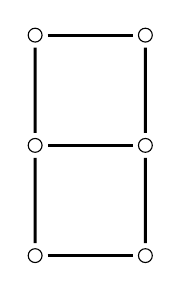
\begin{tikzpicture}
    \begin{scope}[scale=0.7]
      \node (a) at (-1,2)  [vertex]{};
      \node (b) at (-1,0)  [vertex]{};
      \node (c) at (-1,-2) [vertex]{};
      \node (x) at (1,2)   [vertex]{};
      \node (y) at (1,0)   [vertex]{};
      \node (z) at (1,-2)  [vertex]{};

      \foreach \u/\v in {a/b,a/x,y/x,y/b,y/z,c/b,c/z}
        \draw [edge] (\u) to (\v);
    \end{scope}
    \end{tikzpicture}
    \caption{Gr\'afica para el Ejercicio.}
    %\label{fig:choose}
    \end{figure}

    Veamos que la gr\'afica anterior no es coloreable con listas de tamaño dos, el siguiente es un contraejemplo:

  \begin{figure}[ht!]
    \centering
   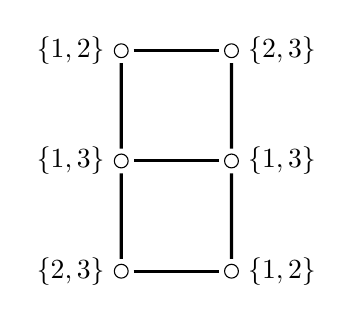
\begin{tikzpicture}
   \begin{scope}[scale=0.7]
     \node (a) at (-1,2)  [vertex, label=180:{$\{1,2\}$}]{};
     \node (b) at (-1,0)  [vertex, label=180:{$\{1,3\}$}]{};
     \node (c) at (-1,-2) [vertex, label=180:{$\{2,3\}$}]{};
     \node (x) at (1,2)   [vertex, label=0:{$\{2,3\}$}]{};
     \node (y) at (1,0)   [vertex, label=0:{$\{1,3\}$}]{};
     \node (z) at (1,-2)  [vertex, label=0:{$\{1,2\}$}]{};

     \foreach \u/\v in {a/b,a/x,y/x,y/b,y/z,c/b,c/z}
       \draw [edge] (\u) to (\v);
     \end{scope}
    \end{tikzpicture}
  \end{figure}

   Se puede ver que \'esta asignaci\'on de listas es imposible de satisfacer suponiendo que el v\'ertice superior izquiero recibe el color $1$ \'o $2$, en ambos casos se llegan a conflictos en la coloraci\'on de otro v\'ertice.

   Ahora, veremos que cualquier asignaci\'on de $3$-listas funciona, considere las siguientes listas arbitrarias:

   \begin{figure}[ht!]
     \centering
     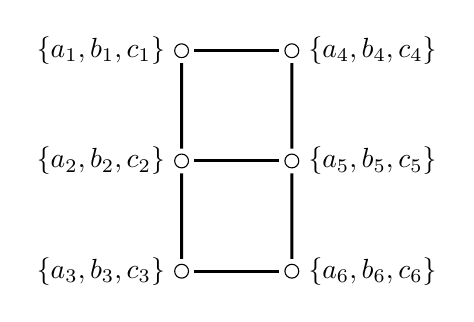
\begin{tikzpicture}
     \begin{scope}[scale=0.7]
       \node (a) at (-1,2)  [vertex, label=180:{$\{a_1,b_1,c_1\}$}]{};
       \node (b) at (-1,0)  [vertex, label=180:{$\{a_2,b_2,c_2\}$}]{};
       \node (c) at (-1,-2) [vertex, label=180:{$\{a_3,b_3,c_3\}$}]{};
       \node (x) at (1,2)   [vertex, label=0:{$\{a_4,b_4,c_4\}$}]{};
       \node (y) at (1,0)   [vertex, label=0:{$\{a_5,b_5,c_5\}$}]{};
       \node (z) at (1,-2)  [vertex, label=0:{$\{a_6,b_6,c_6\}$}]{};

       \foreach \u/\v in {a/b,a/x,y/x,y/b,y/z,c/b,c/z}
         \draw [edge] (\u) to (\v);
     \end{scope}
     \end{tikzpicture}
   \end{figure}

   Nos referiremos a los v\'ertices como $v_1,v_2,v_3,v_4,v_5,v_6$ respectivamente en coherencia con los \'indices de las listas.

   Veamos que si para $v_2$ se elige $a_2$, entonces los v\'ertices $v_1,v_5,v_3$ seguro tienen colores disponibles en sus listas pues \'estos conforman un conjunto independiente y por lo tanto su elecci\'on s\'olo estar\'ia restringida a por $a_2$. Finalmente veamos que como $v_4$ y $v_6$ son adyacentes s\'olo a dos v\'ertices, entonces seguro es posible elegir un color en sus listas que no cause conflictos.

   Con \'esto conclu\'imos que \'esta gr\'afica es $3$-coloreable por listas.

\end{enumerate}

\end{document}
